\documentclass[10pt, a4paper, twocolumn]{article}
\usepackage{graphicx}
\usepackage{enumitem}
\usepackage{fancyvrb}
\title{Meltdown and Spectre}
\author{Began Bajrami, Rahmi El Mechri}
\begin{document}
\maketitle
\begin{abstract}
With this paper we want to make easier to understand what Meltdown and Spectre vulnerabilities are and how they work.
\end{abstract}
\section{Introduction}
With this paper, we want to make easier to understand what Meltdown and Spectre vulnerabilities are and how they work.


\chapter{Out of Order Execution}
% what is out of order?
Out of order is a technique used by many CPUs nowadays and the main reason being the improvements on perfomance that it brings, allowing
CPU to decide what to execute first and what after basing its decision purely on what dependencies the instruction has.


\section{Side channel}
Usually, CPUs support virtual address spaces to isolate processes from each other and to let
compilers use logical addresses instead of directly accessing physical memory addresses.
Virtual addresses are then translated to physical addresses. For optimization of memory usage, paging is also used
to reduce memory usage and to separate User Space addresses from Kernel Mode addresses,
in order to let only privileged processes to access kernel address space. Translation tables are used in order to define virtual to phisical mappings
and also protection properties such as readable, writeble, executable and whether the page is accessible by
user or not (meaning that only kernel mode processes can access the page).
These attributes are verified everytime an instruction is accessing them, resulting in a CPU trap (hardware exception) if the processes
which required that address is not allowed to. This is handled by the Reorder Buffer on superscalar/superpipelined processors, when reordering results
of instructions that have been executed out-of-order.
Every process has its own translation table which is held on a special CPU register, so "on each context switch the \textbf{operating system} updates
this register with the next process' translation table address in order to implement per process virtual address spaces".
Each virtual address space itself is split into a user and a kernel part.

\subsubsection{Exploitation and mitigation}
Attacks that are targeting memory corruption bugs often requires the knowledge of addresses of specific data.
ASLR mitigation has been introduced to randomize address space layout in order to obfuscate memory mapping to
attackers. KASLR (Kernel Address Layout Randomization) was introduced to protect the kernel, randomizing the offsets where
drivers are located on every boot, making attacks harder as they now require to guess the location of kernel data structures.
But KASLR is not sufficent to mitigate Meltdown attacks since a simple bruteforcing of the memory physical addresses can leak
such information.

\subsubsection{What is side-channel}
From Wikipedia, here's a definition of side-channel attack
\begin{quotation}
    In computer security, a side-channel attack is any attack based on extra
    information that can be gathered because of the fundamental way a computer
    protocol or algorithm is implemented, rather than flaws in the design of the
    protocol or algorithm itself or minor, but potentially devastating, mistakes
    or oversights in the implementation.
\end{quotation}
Side channel attacks allows leaking of sensible information, like what pages a processes has recently accessed. These attacks
allow detection of the exact location of kernel data structures or derandomize ASLR. Moreover, software bugs and the knowledge of these addresses
can lead to privileged code execution.

\subsubsection{How is side channel implemented}
More in depth on side channels, there are many ways we can gather information, for example: timing, RF, electromagnetic emissions, and others.
In our case, simply monitoring the time a cache lines needs to reload leaks information about wether this information was in fact already loaded or not.
\subsubsection{Covert channels}
Covert Channel attacks are a special use case of side channels, where basically we intentionally send information
to a system in order to induce the side effects we want to measure.
Specifically for our use case, side channels includes: Evict+Time, Prime+Probe and Flush+Reload. We will discuss only the latter since, as stated by
Meltdown researchers, this is the faster and the more reliable way of doing it.
These attacks are specifically designed to leak information from the cache exploiting timing differences induced by them selfs.

\subsubsection{Flush+Reload}
Flush+Reload is a variant of the Prime+Probe technique  where an attacker
frequently flushes a targeted memory location using the clflush (cache line flush) instruction. By measuring the time it takes to Reload
the data, the attacker determines wether data was loaded into the cache by another process in the meantime.
An attack consists of three phases: first, the attacker flushes the memory cache line that he wants to monitor, then, he just waits for the victim process to read the same
memory line; if the victim has, in fact, accessed that same memory line again, the value will be stored on the cache, otherwise no cache line will be loaded. Which brings
the attacker to the third phase: if the cache line was loaded, the access time to that line will be very fast, otherwise the attempt will result on a "cache miss" which
means that the victim process didn't access to the memory line again (in other words: the attacker will wait much longer to access that value). Usually, the unit measure
used is "cycles the CPU needs to fetch the data" instead of microseconds or any othe time measure.
Meltdown and Spectre attacks use this technique to know what is the value of the secrets the attacker
wants to leak from a specified process or a specified physical memory range.

\section{Speculative Execution}
Speculative execution is a technique implemented by the majority of modern CPUs to maximize perfomances. 
As the name suggests, it is based on the execution of operations that might or might not be performed. The entity that predicts wether or not a certain instruction path, called branch, will be taken is called Branch Predictor.

\subsection{Branch Prediction}
A signifcant number of implementations of branch prediction have been designed over the last 50 years, many of which are the evolution of previously designed 
For the sake of this paper we will just differentiate between 2 of them, more precisely 2 macro-categories of branch prediction.
\subsubsection{Static Branch Prediction}
Static Branch Prediction is the simplest type of Branch Prediction. It utilizes information gathered before the execution of the program.
\subsubsection{Dynamic Branch Prediction}

\subsection{Branch Target Prediction}
Another type of speculation implemented in modern CPUs is Branch Target Prediction.
Indirect jumps are jump instructions where the target address is not directly passed, a register or a memory address containing the target is given instead.
This means that once the CU decodes the indirect jump instruction, clock cycles are spent to fetch the address from the register, cache or, worst-case scenario, a cache-miss happens and the target is fetched from main memory.
To fasten up this process, in order to fetch the target instruction as soon as possible, modern CPUs implement what's called a Branch Target Predictor.
Branch Target Predictor uses a buffer called BTB(Branch Target Buffer), which structure is analog to a cache: it associates instruction PCs to branch target PCs. Every time a new indirect jump is fetch and decoded, its PC and target address are stored in the BTB.
For every entry in the table 2 predictions bits are added, just like branch prediction 2-bit schema, to improve target prediction.
This means that new entry have 2 prediction bits set as 'Predict Taken'.
Every time an instruction is fetched, the BTB is looked up to check if it contains the instruction PC, if so, then the associated target address is sent out.
If it target turns out to be correct ...
If not the entry is deleted from the BTB, and 2 cycles are lost.
If the instruction PC is not in the BTB, if after being decoded turns it's an jump instruction then its PC and target address are saved in the table.
Workflow can be seen in Figure underneath:
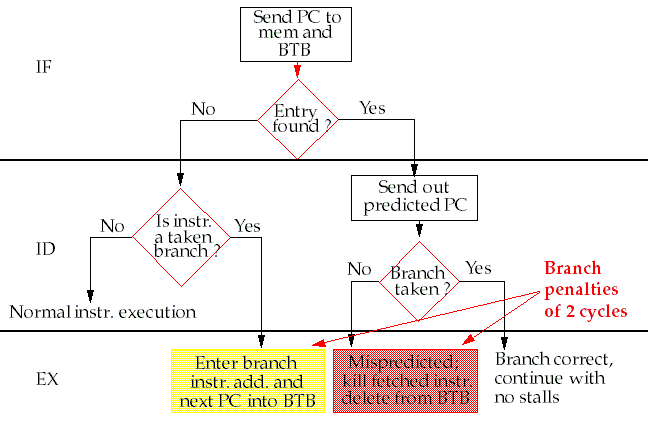
\includegraphics[scale=0.35]{img/BTB.png}



\section{Meltdown}
In this section we will explain how Meltdown attack works and how we managed to
test it on our machines. This paper has the target of explaining how Meltdown works in a more "human readable" manner, and so we will provide pseudocode.

\subsection{How it works}
Meltdown attacks consists of 4 main steps:

\textbf{Step 1} Load content of (inaccessible) memory location on a register

\textbf{Step 2} Allocate "Probe Array" on main memory

\textbf{Step 3} Use the previosly loaded data to transimt secret on a legitimate instruction execution

\textbf{Step 4} Store leaked secret on main memory leveraging Flush+Reload and previosly allocated Probe Array

\subsubsection{Step 1: Fetch privileged data}
Meltdown's main objective is to get privileged data from main memory which is otherwise inaccessible, and to do so
the attack starts with simple access to an unauthorized memory location.
In our example we will refer to such address as the "0xABC0" memory address, which our code is not autorized to access to,
which points to the first byte of an array containing our secret ("Meltdown").
So our secret is stored from "0xABC0" (`m', first letter) to "0xABC7" (`n', last letter).

\begin{Verbatim}[fontsize=\small]
...
   secret = readAddress(0xABC0);
...
\end{Verbatim}
\begin{figure}[!h]
    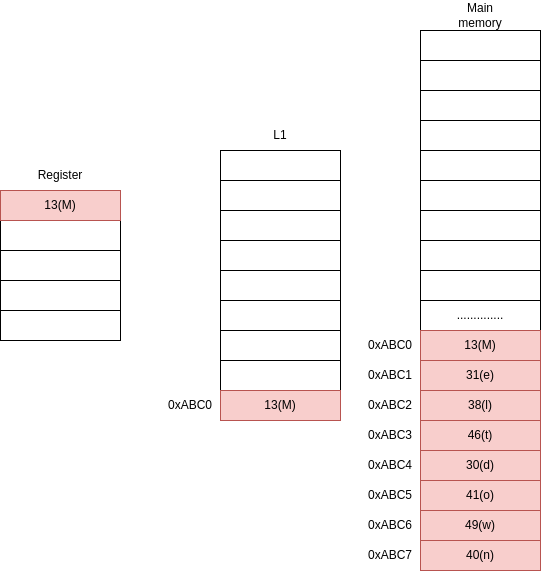
\includegraphics[scale=0.25]{img/meltdown-step-one.png}
    \caption{Current microarchitectural state}
\end{figure}

\subsubsection{Step 2: Allocate Probe Array}
In our example, we allocate a so called Probe Array which holds an array of "acceptable" values for our secret.
\begin{Verbatim}[fontsize=\small]
...
    secret = readAddress(0xABC0);
    probe_array=no_cache_array("A",
	"B", "C",..., "Z", "a", ... "z");
...
\end{Verbatim}
For the sake of simplicity, no\_cache\_array is a function that allocates an array without caching and returns its address.
For example, accessing to probe\_array[2] will result, at current micro-architectural state, in a "cache miss".
This is a fundamental step for out-of-order exploitation.
On the flush+reload step, what we want is that none of the pages holding these data is loaded but the one which store the value
"M" since it is the first char of the secret value.

\subsubsection{Step 3: Transmit secret}
Now we have a register containing the value of the accessed secret and an array that contains all possible values that secret may be equal to,
all is left to do is to legitimately get that value in order to store it on the main memory without the Reorder Buffer deleting its result
after realizing that we should have not accessed that location genearting an architectural exception (also called "trap").

\begin{Verbatim}[fontsize=\small]
...
    secret = readAddress(0xABC0);
    probe_array=no_cache_array("A",
	"B", "C",..., "Z", "a", ... "z");
    probe_array(secret);
...
\end{Verbatim}

What we oversimplified on Line 3 is what loads the desired page on our core cache. On a micro-architectural level, accessing the secret-th value of probe\_array
will first result on a "cache miss" and then the processor loads the value from main memory into the cache.
Note that the pseudocode we provide dosen't really make sense from a more realistic point of view, since we are assuming that the address "0xABC0" is storing the exact
offset in which the value is stored on our probe\_array. In a more realistic example we should first load the value on a register, e.g. RAX,
and then translate that value in something that can be used to retrive a specific page from the memory which,
like hashing functions, is equal to a well-known value. Also, an important note here is that each page
of probe\_array contains exactly and only a single value, being "A" for the first page, "B" for the second, and so on until "z".

\subsubsection{Step 4: Flush+Reload to store the value}
At this point all that's left to do is to store the secret value in a manner that Reorder Buffer will not delete its result.
\begin{Verbatim}[fontsize=\small]
...
    secret = readAddress(0xABC0);
    probe_array=no_cache_array("A",
	"B", "C",..., "Z", "a", ... "z");
    probe_array(secret);
    for(i = 0; i < 52; i++){
        cycle_count_set(0);
        probe_array(i);
        if(cycle_count_get < 100)
            p = probe_array(i);
        clflush(probe_array(i))
    }
...
\end{Verbatim}

\begin{figure}[!h]
    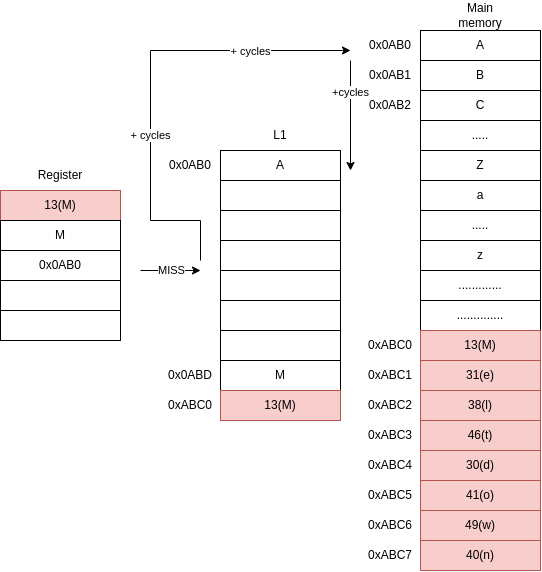
\includegraphics[scale=0.25]{img/meltdown-step-two.png}
    \caption{Microarchitectural state on cache miss}
\end{figure}
\begin{figure}[!h]
    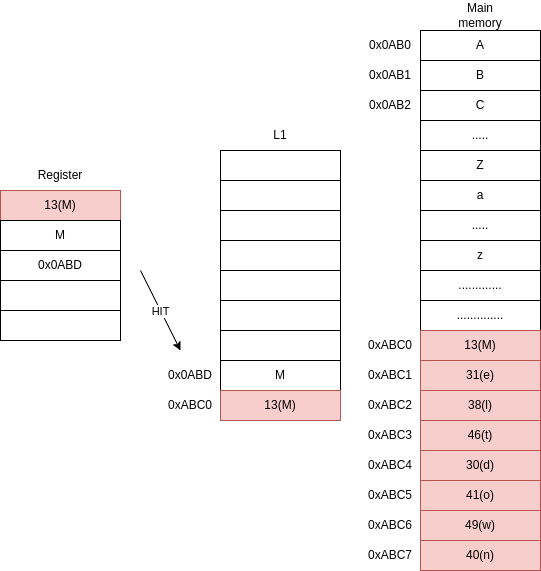
\includegraphics[scale=0.25]{img/meltdown-step-four.png}
    \caption{Microarchitectural state on cache hit}
\end{figure}

In our example, we iterate every page relevant to our probe\_array in order to leverage Flush+Reload technique previously discussed.
We iterate all 52 pages of the probe\_array and measure how many cycles it takes to load the value: we assume that if the cycle count
is lesser than 100, then the page was already cached, which means that line 3 was the last and the only who could have done that.
We now procede to save the value on a register which will not be ereased by the Reorder Buffer since Line 7 is not doing anything wrong
from his point of view. On Line 8 we flush the cache line so to leave pages of probe\_array unloaded until we read the next privileged address.

\subsection{The importance of Transient Instructions}
The Meltdown attack is possible only because these instructions are executed out-of-order.
Subsequent instructions that are executed earlier than intended are called transient instructions.
As previously discussed, instructions accessing privileged addresses are not denied by the CPU even if the process is not allowed to: there's
another mechanism handling the privileged access to these information, meaning instructions are executed regardless of their privilege but their result will raise an
exception.
Exceptions are in fact raised by Meltdown, but handled so that the program continues its execution regardless.
A trivial approch is to fork the attacking application before accessing invalid memory location, so that when exception raises the child program crashes, but the parent
can still observe the microarchitectural state, e.g. through a side-channel.
Another way of handling exceptions is to suppress them thourgh Intel TSX which allows to group multiple instructions to a "transaction", which appears to be an
atomic instruction. If one instruction within the transaction fails, already exectuted instructions are reverted, but no exception is raised. The microarchitectural effects
are still visible.

\section{Spectre}
Spectre vul
\subsection{Spectre v1 - PHT}
\subsection{Spectre v2 - Branch Target Injection}
\subsection{Spectre v3 - RSB}
\subsection{Spectre v4 - STL}

\input{mainmatter/5-meltdown-exploit.tex}
\input{mainmatter/5-spectre-exploit.tex}
\input{mainmatter/7-stats.tex}
\section{Meltdown mitigations}
Since Meltdown is a micro-architectural vulnerability, there is no software update that can completely make mahcines secured from Meldown attacks.
Not even KAISER (also known as PTI, page-table isolation, or KPTI on Linux kernel) which is the proposed
mitigation by meltdown researchers make machines secure. That's because
Meltdown, and Spectre, acts on hardware and bypasses the hardware-enforced isolation of security domains.
A countermeasure would be to completely disable out-of-order execution but this will make processors slow enough to make any modern CPU parallelism mechanism
completely useless and the performance impact would be devastating. As of 2022, PTI (KAISER) is enabled by default on Linux kernels as a countermeasure to Meltdown.

\subsection{KAISER}
KAISER (Kernel Address Isolation to have Side-channels Efficiently Removed) was not originally intended for Meltdown, but has as side effect the mitigation of it
since KAISER prevents side channel attacks breaking KASLR. But this has its own limitations: first of all, performances will decrease since every context switch will
need more clock cycles for address mappings; second, there is still a residual attack surface for Meltdown since several privileged memory locations are required
to be mapped in user space. However, these memory locations do not contain any secrets, but they might contain pointers to Kernel Address space. This information, if leaked,
is enough to break KASLR, as the randomization can be calculated from the pointer value.

\section{Spectre Mitigations}
In this section we will discuss the different countermeasures proposed for the Spectre vulnerability.
\subsection{Speculative Execution Prevention}
As stated multiple times, Spectre totally relies on Speculative Execution. 
Removing it would eliminate the vulnerability, but it would also mean renouncing to decades of performance improvement, therefore making this solution impracticable.
AMD and Intel suggested, as software solution, using the lfence instruction, that doesn't allows instruction following it to be executed.
In practice this means renouncing to speculative execution, hence should be used only when transient instructions could lead to dangerous otucomes.
\subsection{Secret Data Access Prevention}
Spectre vulnerability can be exploited using code written in JavaScript, thus browser, can and have to implement solutions to make the access to secred data more difficult.
Google Chrome runs every website on a separate process as certain Spectre exploits are limited by victim permissions.
Webkit implements 2 solutions: replaces array bounds checking with index masking, and xores pointers with pseudo random poison value.
The first limits bounds violation, the latter prevents attackers that don't know the poison value to access those pointers.
\subsection{Limiting Covert Channel}
As all spectre variants use covert channels, limiting their exploitability is crucial.
The researchers that discovered Spectre suggest that future processors could track if data was fetched by a transient instruction and prevent it to be leaked by limiting the number of operations that can be performed on it.
Another way to limit covert channel is making known side channels harder, such ad the approachtaken by different browser that downgraded JavaScript timer, therefore making time-based side channels less efficient.
\subsection{Branch Poisoning Prevention}
Intel and AMD have implemented different mechanisms to prevent Branch Poisoning, released with a microcode patch extending the ISA: Indirect Brnach Restricted Speculation(IBRS), Single Thread Indirect Branch Predictio(STIBP) and Indirect Brnach Predictor Barrier(IBPB).
IBRS prevents cross-privilege Branch Target Prediction mistraining, by isolating the BTB based on privilege. A similar mechanism is implemented by ARM's CSV2.
STIBP limits the influence on branch predictor caused by thread running on the same core.
IBPB prevents software running before a certain moment from influencing software executed after it.
These mechanisms require OS support.
Google suggests a mechanism, called retpolines, that replaces indirect branches with return instructions, and implementing a benign infinite loop to prevent speculation of indirect branches.

\section{Conclusions}
The discovery of Spectre and Meltdown vulnerabilities demonstrated that the neverending run for higher perfomances must be backed up by a thorough security check on what type of exploits this can lead to. 
Four years passed since their discovery, and researchers still find new ways to leverage speculative execution.
It is clear that a Spectre-and-Meltdown-proof CPU is still far from being achieved, but a positive side effect is that the research for new microarchitectural bugs has been incentivized, and this resulted in the recent discovery of PACMAN vulnerability in new M1 chips.

\newpage
\section{References}
\begin{itemize}
    \item https://meltdownattack.com/meltdown.pdf
    \item https://spectreattack.com/spectre.pdf
    \item https://www.cs.cmu.edu/afs/cs/academic/class/15740-s17/www/lectures/L19-BranchPrediction.pdf
    \item https://web.archive.org/web/20190717130447/http://web.engr.oregonstate.edu/~benl/Projects/branch\_pred
    \item https://ece-research.unm.edu/jimp/611/slides/chap4\_5.html
    \item https://www.usenix.org/system/files/conference/woot18/woot18-paper-koruyeh.pdf
    \item https://www.cs.umd.edu/~meesh/411/CA-online/chapter/dynamic-branch-prediction/index.html
    \item https://docs.oracle.com/cd/E23824\_01/html/819-3196/hwovr-14.html
    \item https://www.redhat.com/en/blog/speculative-store-bypass-explained-what-it-how-it-works
    \item https://www.techrepublic.com/article/spectre-and-meltdown-explained-a-comprehensive-guide-for-professionals/
    \item https://course.ece.cmu.edu/~ece740/f15/lib/exe/fetch.php?media=18-740-fall15-lecture05-branch-prediction-afterlecture.pdf
    \item https://download.vusec.net/papers/bhi-spectre-bhb\_sec22.pdf
    \item https://www.usenix.org/sites/default/files/conference/protected-files/woot18\_slides\_koruyeh.pdf
    \item https://gruss.cc/files/kaiser.pdf
    \item https://www.youtube.com/watch?v=D1DNz5sNDgE
    \item https://en.wikipedia.org/wiki/Covert\_channel
    \item https://www.usenix.org/system/files/conference/usenixsecurity14/sec14-paper-yarom.pdf
\end{itemize}

\end{document}
